% IEEE standard conference template; to be used with:
%   spconf.sty  - LaTeX style file, and
%   IEEEbib.bst - IEEE bibliography style file.
% --------------------------------------------------------------------------

\documentclass[letterpaper]{article}
\usepackage{spconf,amsmath,amssymb,graphicx}
\usepackage{graphicx}
\usepackage{tabularx}
\usepackage[export]{adjustbox}
\usepackage{float}
\usepackage{array}
\usepackage{amsmath}
\usepackage{algorithm}
\usepackage[noend]{algpseudocode}

\usepackage{subcaption}


% Example definitions.
% --------------------
% nice symbols for real and complex numbers
\newcommand{\R}[0]{\mathbb{R}}
\newcommand{\C}[0]{\mathbb{C}}

% bold paragraph titles
\newcommand{\mypar}[1]{{\bf #1.}}

% Title.
% ------
\title{Predictions of urban qualities in the city of Zurich}
%
% Single address.
% ---------------
% \name{Jakub Lichman, Philippe Schlattner, Florian Koch}
% \address{Department of Computer Science\\ ETH Zurich\\Zurich, Switzerland\\\\ Email: \{lichmanj, pschlatt, flkoch\}@student.ethz.ch}

% For example:
% ------------
%\address{School\\
%		 Department\\
%		 Address}
%
% Two addresses (uncomment and modify for two-address case).
% ----------------------------------------------------------
%\twoauthors
%  {A. Author-one, B. Author-two\sthanks{Thanks to XYZ agency for funding.}}
%		 {School A-B\\
%		 Department A-B\\
%		 Address A-B}
%  {C. Author-three, D. Author-four\sthanks{The fourth author performed the work
%		 while at ...}}
%		 {School C-D\\
%		 Department C-D\\
%		 Address C-D}
%

\twoauthors
 {Jakub Lichman, Philippe Schlattner}
		 {Department of Computer Science}
 {Florian Koch}
		 {Department of Physics}

\address{\\ETH Zurich\\Zurich, Switzerland\\Email: \{lichmanj, pschlatt, flkoch\}@student.ethz.ch}

\begin{document}
%\ninept
%
\maketitle
%

\begin{abstract}
We should do as the last one.
\end{abstract}

\section{Introduction}\label{sec:intro}
Huge predicted increase in the number of world urban area residents from 54 to 66 percent in 2050 brings many challenges
which every successful city has to overcome. Cities of the future have to ensure continuous improvement of their
services despite growing population. Since it is impossible for a city to reach excellence in all services,
authorities have to aim for compliance in a prioritised subset of its services. For instance, this year's Mercer's Quality of Living index\cite{mercer}
takes into account economic and political environment, infrastructure, public transport, health, recreation and housing
to decide which cities are the most desirable. Based on these factors, the list of most liveable cities was constructed.
However, these types of rankings usually generalise the whole city and take average of all the districts which can
over or underrate them. In our paper we tried to distinguish urban qualities within a city, concretely in the city of Zurich.
Its public data availability enabled us to make interesting predictions about urban qualities of the individual city districts
which we lately verified by examining selected places in person.

\indent Our experiment tries to exploit data that is publicly available for the city of Zurich as well as data that we tried to obtain ourselves.
The goal was to create a map of the city with multiple layers where each layer will represent one factor of urban quality. By summing all factors and
visualising them we can obtain an interactive map which visualises liveability of each part of the city. Later we evaluated selected areas with the Smart
Agora platform which enabled us to collect data for validation by walking in these areas.

\indent The main contribution of this paper is to automate reasoning about urban qualities. Nowadays it is done by
real estate agents which charge big amounts of money for such services. In the future their jobs can be
completely automated and so computers will monitor urban qualities and suggest accommodation prices as well as
provide sets of possible actions to improve quality of life in poorly rated locations.

\mypar{Related work} This paper is mainly based on the previous work of Danielle Griego et al. \cite{smartCities}
where an internet of things approach is used to obtain the citizen's perception of the selected areas of the city of Zurich.
Paolo Neirotti et al. \cite{smartCities2} in their paper provide comprehensive understanding of the notion of a smart city
through the elaboration of natural resources and energy, transport and mobility, buildings, living, government, economy
and people. Kunwar P. Singh et al. \cite{pollution} used principal components analysis (PCA) to identify sources
of pollution and tree based learning models to predict the urban air quality of Lucknow (India) using the air quality
and meteorological databases.
\\
\indent This paper is organised as follows: Section~\ref{sec:background} explains what a smart city is, its history, tools that are used
in smart cities and its practical applications in the praxis. Section~\ref{sec:data} describes the data that were used for our
experiment and their sources. Section~\ref{sec:attractiveness} defines the criteria by which we will rate the locations within Zurich.
Section~\ref{sec:greenery} explains greenery detection process in our approach and Section~\ref{sec:predictions} describes method of creating the quality index
map of the city. In Section~\ref{sec:exp} the predictions are evaluated through the Smart Agora platform. Finally, Section~\ref{sec:discussion} concludes this
paper and outlines future work.

\section{Background}\label{sec:background}
The term "Smart Cities" has attracted recently \cite{Ferdowsi2018,Abu-Matar2018,Usman2018} some attention. It is usually referring 
to the real time analysis of whole cities and their population \cite{smartCities3}. It can also imply economical 
innovation which is usually equated with entrepreneurship created by smart people.\\
\indent In the process of establishing this expression, two main  sources of data have been identified \cite{smartCities3}. 
On the one hand this compromises the increasing number of stationary installed computer connected hardware, such as traffic cameras, 
telecommunication networks and building management systems. On the other hand the population carries an even faster increasing 
number of mobile computers like smart phones, navigation systems or even fully connected vehicles.\\
\indent By combining these data sources and analysing them in the real-time, one is able to not only steer the flow within a city 
but also predict the evolution. The Chinese central government has recently been attracted by the media \cite{thediplomat1} for not only 
using the public surveillance system to track down criminals but also equip the police officers with glasses that have an integrated 
cameras \cite{cnet1}. According to the same article, they plan to have a public credit system in place for all its 1.4 billion citizens 
by 2020, which will be crucial for obtaining jobs or getting permission to travel abroad.\\
\indent The real time analysis of their currently over 170 million CCTV cameras \cite{bbc1} enabled them to arrest a suspect, who was 
identified by facial recognition amongst 60'000 visitors to a concert. These are just a few examples of how the connection between various 
data sources enables people having access to the data to widely control public live.\\ %this sentence is not that good
\indent It also points out some of the threats. With the public credit and shame system \cite{cnet1} everyone has to constantly 
adhere to the accepted code of conduct in order to not loose points or be publicly denounced. This ubiquitous surveillance is feared 
by many privacy policy activists, slowing down similar efforts in western countries. In the end we will have to decide in which kind 
of world we all want to live in.\\
\indent However the thus obtained data can also be used for the good. Responsive traffic management systems are a necessity in current 
megacities, where an increasing number of cars tries to reach their destination on roads that cannot be extended any further. 
And also the public transport systems reach their limits when an ever increasing number of people tries to get from the point A to the point B 
all at the same time. Wisely employed camera systems not only allows to track the flow of people but the correct data analysis promises to resolve 
some of the problems.\\
\indent In our project we tried to use data from various sources to rate the living quality for people within the districts of Zurich. 
As most of the real time data in Zurich is not publicly available, we set out to analyse less fast paced data first. The predictions 
should then be checked with data obtained from study participants, who would walk those areas to collect data with their smart phones. 
In the future expansion this could allow us to assess the living quality not only in general but also for different days of the week or even 
different times of the day.

\section{Data}\label{sec:data}
To begin with, we evaluated data downloaded from the open data initiative of the city of Zurich \cite{ZurichOD}. 
Furthermore, we used maps from the Geographic Information System of the canton of Zurich GISZH \cite{GISZH} 
to get an idea of potentially interesting areas.\\
\indent These two sources were used, since we believed that data published by institutions of the government 
is in general more reliable than that published by individuals. In addition, the data is considered to be of better 
quality and cover more of the area. This initial trust has been partially disappointed by finding quite a few data 
sets with only few points. As we wanted to predict the best living areas within Zurich, we also needed data that covers 
more or less the complete area of Zurich in order to avoid bias towards certain regions, which are better covered 
by the data sources. Therefore, we omitted data sets with subjectively too few entries, which we initially wanted 
to use due to their potential. These omitted data sets include the one on air quality, flat prices and traffic counts.\\
\indent The data we finally used and analysed is composed of records for public street illumination, pedestrian zones, 
sighing points, zones where driving is prohibited as well as restaurants. These are all sets where the available data 
is spread across a large part of Zurich and that we figured might be indicative for how much we as students would 
appreciate living there. This is a highly subjective measure that took us some time to agree amongst ourselves on.\\
\indent The analysis of the data is described in the Section~\ref{sec:predictions}. In addition we inferred the amount 
of greenery from satellite images as outlined in the Section~\ref{sec:greenery} to evaluate how green the urban areas are. 
Finally we tried to evaluate the predictions by having people walk some of the areas and gather their impression 
by utilising Smart Agora. The details of the last bit are outlined in Section~\ref{sec:exp}.

\section{Measure of Attractiveness}\label{sec:attractiveness}
As we are all students at ETH Zurich, we wanted to map the attractiveness to live in a certain area from the student point of view.
Therefore, access to the public transport is crutial. However walking for up to 15 minutes does not bother us that much. Hence, we did not
include stops of the public transportation in our analysis, since they are all distributed well enough and therefore we found a stop in a walking 
distance to each and every location within Zurich.
On the other hand we did not have access to the detailed data on diverse measures. Accordingly we defined spheres of influence for all types
of points we used for our analysis, that should represent how far we believe that item will influence how we perceive the area.
This also means that accessibility is not that relevant, compared to the bars and restaurants. Another factor that is
very important to us is the proximity to places we visit frequently. However, this is even more subjective and even in our
small group of people we could not identify several points of interest, that are common to all of us except for study related locations.

\section{Greenery Detection}\label{sec:greenery}
\indent Greenery has always played a crucial part in the construction of cities. The need for green spaces has been present since ancient times.
City parks are traditional place of recreation and relax for all kinds of people in their spare time. Current trends in the architecture brought new ways of
connecting buildings and greenery such as roofs with green surfaces or terraces with tree pots. These trends are a consequence of the natural
human inclination towards nature. Therefore, we have decided to take greenery as a significant indicator of urban quality.

\indent In order to predict user preferences partially based on a greenery, we needed to acquire data about it. There are two basic ways of detecting trees,
parks or grass areas on a map. First approach relies on a snapshot of a satellite view \cite{smartCities}. It is simple to implement and yields accurate results.
Detection of green areas is via pixels with RGB values that lie within a specified interval. The only crucial requirement in order to have precise detection
is to use high resolution satellite images of the selected area which in our case were taken from the Google maps satellite view.

\indent Second approach is to detect greenery from the Google Street View (GSV) \cite{googleView}. Xiaojiang Li et. al. detected greenery by examining street
pictures taken from GSV. With this method they were able to explore greenery inside the cities in great detail. The idea behind the second method is in general
more accurate since it can detect trees shadowed by taller buildings or shelters. However, its precision highly depends on the availability of street view and
algorithms, which are in our view still not accurate enough. That is the reason why we have decided to use the first method.

\indent We have developed the python script which does greenery detection similar to the first approach mentioned above.
Firstly, we did the transformation of RGBA\footnote{RGBA corresponds to Red, Green, Blue and Alpha, where the first three values lie in the range from 0 to 255 as in usual RGB and $\alpha$ or A gives the opacity in the range from 0=transparent to 1=opaque} pixel format into HSV\footnote{HSV corresponds to Hue, Saturation and Value, where Hue is an angle on the colour wheel, Saturation is the intensity of the colour and Value corresponds to the brightness} one where detection of colour spectrum is more accurate.
However, during searching for the accurate green space range we encountered a few issues. Detection of grasslands together
with forests was infeasible within a single interval. While grasslands are pixels of a bright green, forests are
the ones with a very dark one together with a dark grey in the locations where one tree shadows the other.
Therefore, we had to distinguish between them and thus do two separate detections. Combination of them then
produced the desired result. Detection of forests, grasslands and their combination can be seen in the Figure~\ref{fig:ZurichGreenery}.
Detected locations are marked with the RGB value (0, 200, 0) which is solid green. Furthermore our method computes an intensity matrix
which indicates influence of the detected greenery on every place within the city of Zurich.

\begin{figure}
    \centering
    \begin{subfigure}{.22\textwidth}
        \centering
        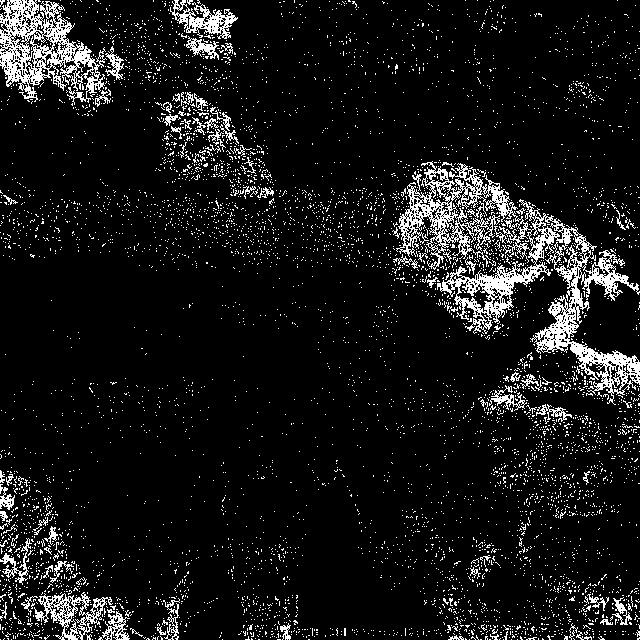
\includegraphics[width=.95\linewidth]{images/greenery/forests.png}
        \caption[width=.2\textwidth]{Mask of the forests}
    \end{subfigure}%
    \begin{subfigure}{.22\textwidth}
        \centering
        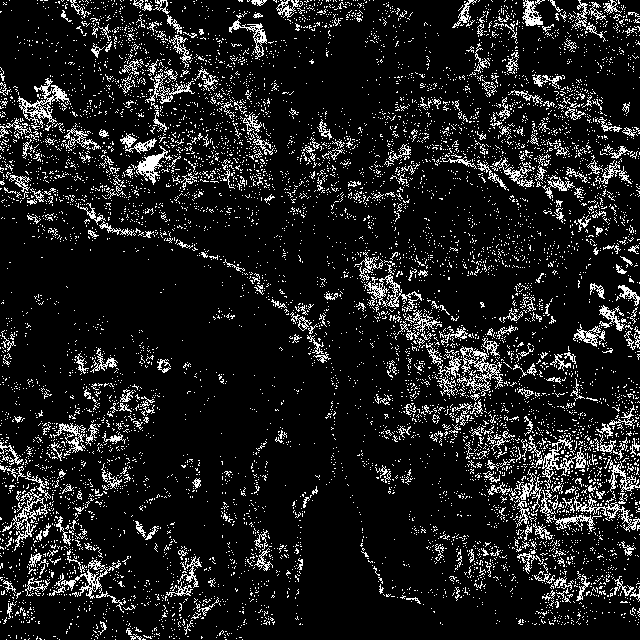
\includegraphics[width=.95\linewidth]{images/greenery/green_areas.png}
        \caption[width=.2\textwidth]{Mask of the grasslands}
    \end{subfigure}

    \begin{subfigure}{.22\textwidth}
        \centering
        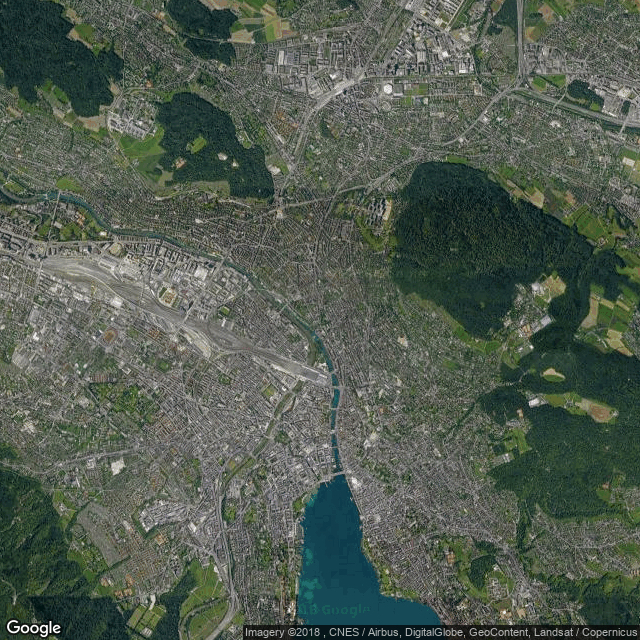
\includegraphics[width=.95\linewidth]{images/greenery/Zurich.png}
        \caption[width=.2\textwidth]{Unmodified Zurich area}
    \end{subfigure}%
    \begin{subfigure}{.22\textwidth}
        \centering
        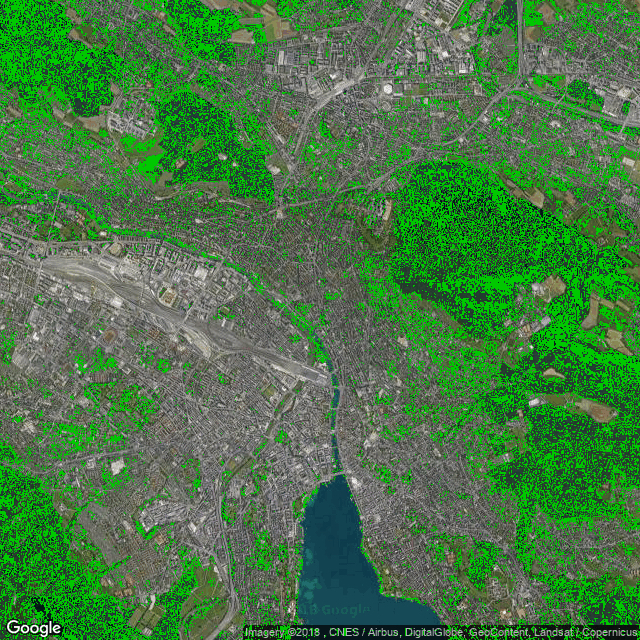
\includegraphics[width=.95\linewidth]{images/greenery/Zurich_greenery.png}
        \caption[width=.2\textwidth]{Greenery in the Zurich area}
    \end{subfigure}
    \caption{Visualization of the greenery detection phases. In the original image we firstly detected forests then
             grasslands and finally we combined them and overlay above the original image.}
    \label{fig:ZurichGreenery}
\end{figure}

\indent Our approach firstly produces a binary matrix $B$ of the image $P$ with greenery locations $G$ such that
\newline
\begin{align*}
B_{i,j} = \begin{cases} 1 & \text{if } P_{i,j} \in G\\
                         0 & \text{if } P_{i,j} \notin G
\end{cases}
\end{align*}
\newline
In the second phase we perform so called "smoothing" of the greenery edges. After the first phase where we have obtained matrix $B$,
we now have to compute the influence of the greenery on the pixels without it i.e. the ones with the value 0. The reason why it is needed is
because inhabitants do not live in the forests or on the meadows but rather profit from living close to them. Therefore, we have
to "influence" pixels that are in the close neighbourhood with the greenery ones. Our algorithm is iterative and so in every iteration
visits every entry in the matrix and checks all neighbouring pixels, finds maxima of them and assigns its half to the current one.
The method can be more formally defined as in Algorithm~\ref{smooth}.

\begin{algorithm}
    \caption{Smoothing}\label{smooth}
    \begin{algorithmic}[1]
        \Procedure{Smoothing}{iterations, B}
            \State $\textit{S} \gets \textit{B}$
            \State $\textit{i} \gets \textit{0}$
            \State $\textbf{while } \textit{i} < 0:$
            \State $\indent \textbf{forall } p \textbf{ in } S:$
            \State $\indent \indent p := max_{neighbours}(p) / 2$
            \State $\indent \textit{i} \gets \textit{i} + 1$
        \EndProcedure
    \end{algorithmic}
\end{algorithm}

The effect of the smoothing Algorithm~\ref{smooth} after 2 iterations on the Matrix~\ref{eq:MatA}
can be seen in the Matrix~\ref{eq:MatB}. Remaining $0$ entries would be replaced by $0.125$ after
the third iteration.

\begin{equation}
\begin{pmatrix}
    0 & 0 & 0 & 0 & 0 \\
    0 & 0 & 0 & 0 & 0 \\
    0 & 0 & 0 & 0 & 0 \\
    0 & 0 & 0 & 1 & 0 \\
    0 & 0 & 0 & 0 & 0 \\
\end{pmatrix}
\label{eq:MatA}
\end{equation}
\begin{equation}
\begin{pmatrix}
    0 & 0 & 0 & 0 & 0 \\
    0 & 0.25 & 0.25 & 0.25 & 0.25 \\
    0 & 0.25 & 0.5 & 0.5 & 0.5 \\
    0 & 0.25 & 0.5 & 1 & 0.5 \\
    0 & 0.25 & 0.5 & 0.5 & 0.5 \\
\end{pmatrix}
\label{eq:MatB}
\end{equation}

\section{Urban quality prediction}\label{sec:predictions}
TODO: This should be "core" chapter of our paper. Philippe here you can describe whole 
procedure of data visualization + correlation matrix etc.

\section{Predictions evaluation}\label{sec:exp}
For evaluating the predictions we derived in the previous section, we chose to let people rate 
that areas based on their visual impression after walking through the respective part of the city. 
For this we initially wanted to use Smart Agora, as it allows to pose the questions at various locations.

Instead we generated a map with markers in various positions and asked people to answer the same questions at those locations. 
Whereas this does not allow to gather additional information, it is more comfortable to use and easier to collect data from 
different people. All participants were asked to answer the five questions, where the first two are single choice 
and the last three are multiple choice questions. The order of the questions was the same for each path but randomly varied 
between different locations. The questions and answer options \ref{app:questions}, locations of the questions \ref{fig:path_points}
and greenery along the walking areas \ref{fig:path_greenery} can be found in Appendix. .

\section{Discussion}\label{sec:discussion}
In this chapter we would like to discuss problems we encountered during our project and outline possible improvements.
\subsection{Smart Agora}
\begin{figure}[htb]
    \centering
    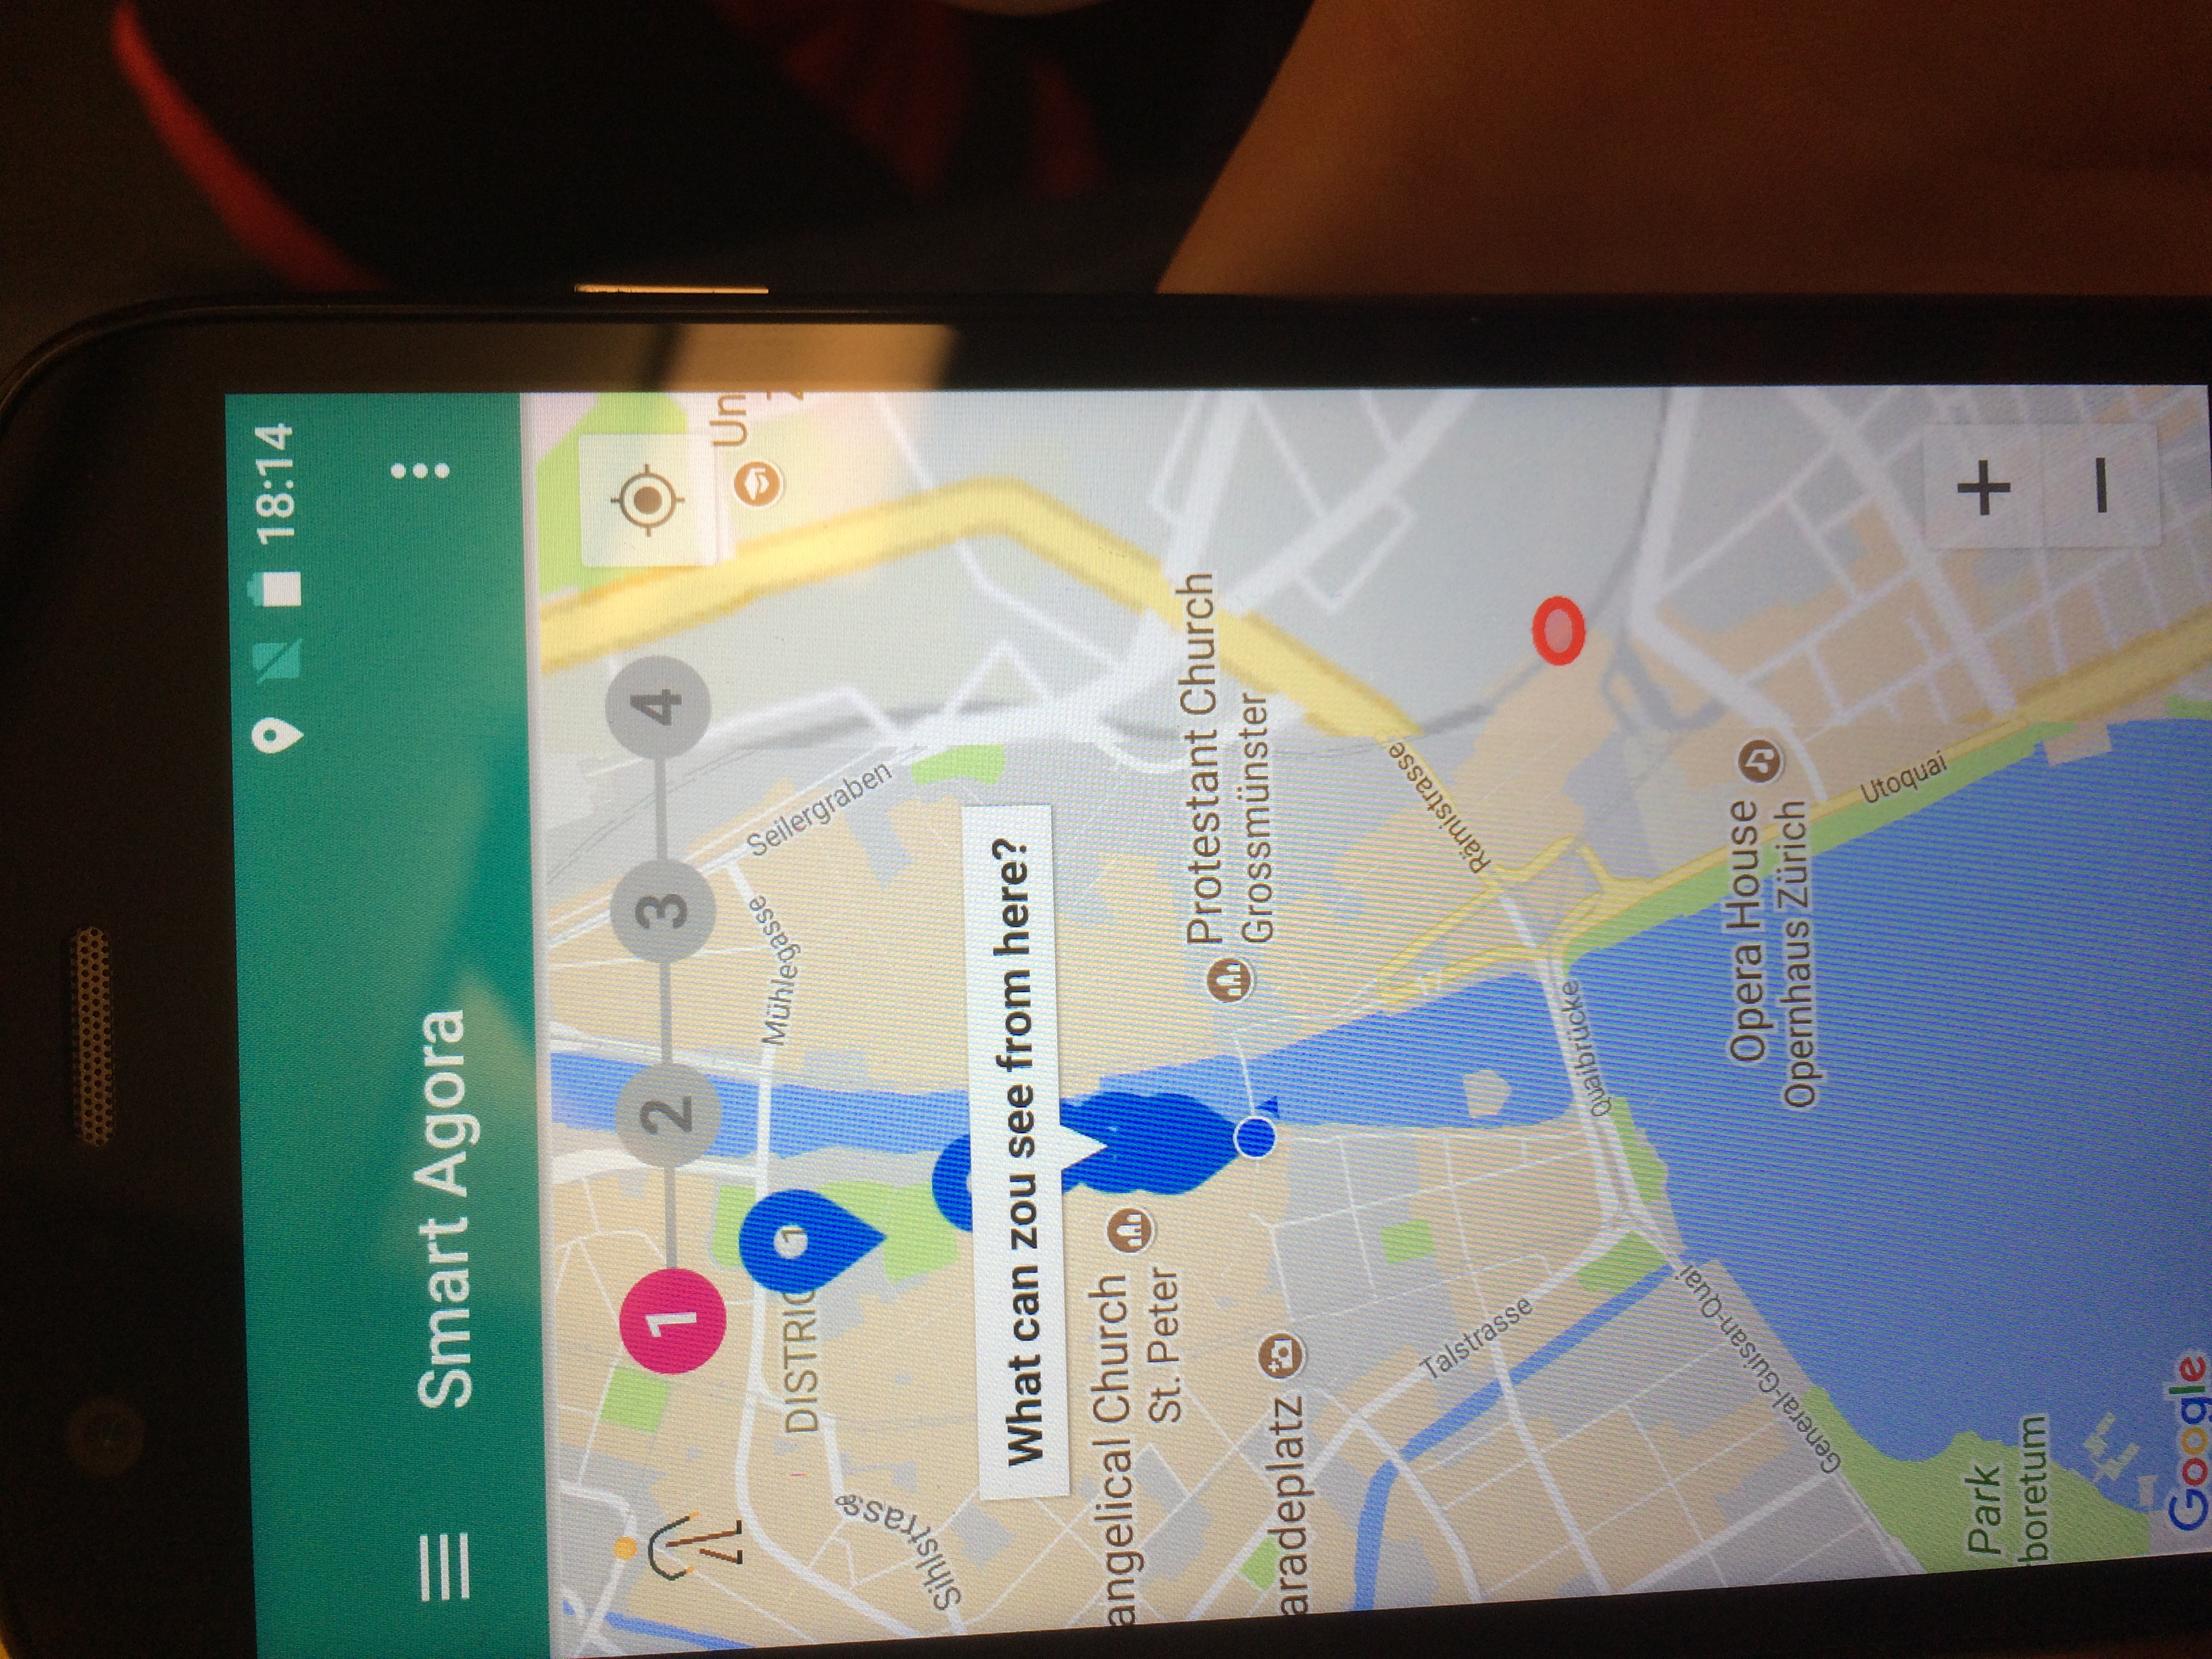
\includegraphics[width=\columnwidth, rotate=270]{images/SmartAgora/img_6.jpg}
    \caption{Smart Agora app with location indicated by the blue dot with arrow and the sphere for answering questions shown in red.}
    \label{fig:smart_agora_1}
\end{figure}
In order to use Smart Agora effectively, we would appreciate the following additions to the platform. Firstly, 
it would be necessary to save parts of a task in case there is a problem with the internet connection 
so we can resume at a later point. Correcting typos would add the app more professional look. For this a preview of the saved tasks is crucial, 
preferably in a more user friendly form than a json file. Also the ability to delete erratic questions after the task was saved 
might be useful, combined with the graciously implemented ability to upload json files directly. Unfortunately the format 
of the data was changed in between, which required us to find the non documented changes and adopt them inside our json files.\\
\indent However using the app was even more troublesome. The generated checkbox questions with seven answers would freeze 
the app on trying to save the selected answers. That is given that the positioning worked correctly
\footnote{cf. Figure~\ref{fig:smart_agora_1} for an erratic localisation} and the pop-up to answer the question actually 
appeared once one arrived at the designated location. Moreover, we would expect to be able to answer the questions in a random order, 
if they were set-up in "Simple" and not in "Sequence" mode. However, a warning appeared after the third question that some had been skipped 
and visiting those locations did not allow us to answer these questions.\\
\indent Occasional crashes of the entire app might be expected in the development phase. However, if non of the entered data 
is stored locally on the phone, this resets every input, including the researcher ID and potentially answered questions. 
This complete data loss, which occurs on every quit of the app, renders any tasks with more than a couple of questions extremely dangerous. 
Even with our short tasks of five questions each, we were not able to complete any of them at the first attempt. This user experience will 
hinder wide spread participation, which would be required for obtaining the collection of larger data sets.

\section{Conclusion}
We should do as the last part together with abstract.


\bibliographystyle{IEEEbib}
\bibliography{bibl_conf.bib} %pick these locations + photos of walking and measured re-

\section{Appendix}
\subsection{Questions for survey}\label{app:questions}
The following questions were asked to evaluate our predictions. After each question one finds the possible answers. 
The first two questions are single choice, whereas the other three are multiple choice. 
The order of questions was the same for each participant, but varied for the different locations.

\begin{enumerate}
	\item Would you like to live hear if you had the opportunity?
	\begin{itemize}
		\item certainly yes
		\item rather yes
		\item rather not
		\item certainly not
	\end{itemize}
	\item Is it likely, you could currently afford a flat in this area?
	\begin{itemize}
		\item certainly yes
		\item rather yes
		\item rather not
		\item certainly not
	\end{itemize}
	\item What do you like about this place?
	\begin{itemize}
		\item It's close to transport.
		\item It's close to shopping.
		\item It's close to other places I often visit.
		\item It's calm with lots of green.
		\item It's visually appealing.
		\item It's bright and open.
		\item It's modern and well maintained.
	\end{itemize}
	\item What do you dislike about this place?
	\begin{itemize}
		\item It's far from transport.
		\item There are no/insufficient shopping possibilities nearby.
		\item It's too far to the places I usually visit.
		\item It's very busy and there are no tree nearby.
		\item It looks ugly.
		\item It's very confined and poorly illuminated.
		\item It's old and shabby.
	\end{itemize}
	\item What can you see from here?
	\begin{itemize}
		\item A stop for public transport.
		\item Parking facilities.
		\item Store for buying food.
		\item A restaurant or a bar.
		\item Construction site.
		\item A park.
		\item A nice flat that I could live in.
	\end{itemize}
\end{enumerate}

\subsection{Images}
\begin{figure}[htb]
    \centering
    \includegraphics[width=\columnwidth]{images/greenery/Zentrum_greenery.png}
    \caption{Greenery detection in the area of our path.}
    \label{fig:path_greenery}
\end{figure}

\begin{figure}[htb]
	\centering
	\includegraphics[width=\columnwidth]{images/greenery/Zentrum_path.png}
	\caption{Locations of question points along the path}
	\label{fig:path_points}
\end{figure}
\end{document}
